\chapter{Progetto 1 bis: Mini libreria per sistemi lineari}
\section{Introduzione}
Per la realizzazione della libreria contenente i metodi iterativi per la risoluzione
di sistemi lineari, è stato scelto di utilizzare \href{https://julialang.org/}{\textbf{Julia}},
un linguaggio di programmazione open-source, sviluppato per ottenere prestazioni
elevate e con una sintassi simile a quella di Python e MATLAB. Essendo concepito
per risolvere task relativi al calcolo scientifico, offre una vasta gamma di
librerie per la gestione di matrici e vettori.

In particolare, per lo sviluppo di questo progetto sono state utilizzate due
librerie della Standard Library di Julia:
\begin{itemize}
    \item \textbf{LinearAlgebra}: fornisce funzioni per la manipolazione di
          matrici e vettori.
    \item \textbf{SparseArrays}: fornisce funzioni per la gestione di matrici sparse.
\end{itemize}

L'impiego di quest'ultima libreria è stato fondamentale per ridurre l'occupazione
di memoria, in quanto le matrici utilizzate negli esperimenti sono matrici sparse.
Nello specifico, sono state utilizzate le seguenti matrici:
\begin{table}[!ht]
    \centering
    \resizebox{\textwidth}{!}{\begin{tabular}{@{}ccccccc@{}}
            \toprule
            \rowcolor[HTML]{EFEFEF}
            \textbf{}      & \textbf{Dimensione} & \textbf{\# Elementi nulli} & \textbf{Condizionamento} & \textbf{Simmetrica} & \textbf{Definita positiva} & \textbf{Dominanza diagonale} \\ \midrule
            \textbf{spa 1} & 1000 x 1000         & 182434                     & 2048.15                  & Si                  & Si                         & No                           \\
            \textbf{spa 2} & 3000 x 3000         & 1633298                    & 1411.97                  & Si                  & Si                         & No                           \\
            \textbf{vem 1} & 1681 x 1681         & 13385                      & 324.64                   & Si                  & Si                         & No                           \\
            \textbf{vem 2} & 2601 x 2601         & 21225                      & 507.02                   & Si                  & Si                         & No                           \\ \bottomrule
        \end{tabular}}
    \caption{Caratteristiche delle matrici utilizzate. Con dominanza diagonale
        si intende quella stretta e per righe.}
\end{table}

\begin{nota}
    Le matrici Vem1 e Vem2 sono a dominanza diagonale non stretta per righe, il
    che non rispetta l'ipotesi di convergenza dei metodi di Jacobi e Gauß-Seidel.
\end{nota}

Per permettere la riproducibilità degli esperimenti, vogliamo riportare di seguito
le caratteristiche del sistema utilizzato per la realizzazione della libreria e
per l'esecuzione degli esperimenti. Tutti gli esperimenti sono stati eseguiti su
un computer con le seguenti caratteristiche:
\begin{itemize}
    \item CPU: Intel Core i5-1135G7
    \item RAM: 16 GB
    \item Sistema Operativo: Windows 11
    \item Julia: versione 1.10.2
\end{itemize}
\section{Struttura della libreria}
La libreria realizzata è composta da tre moduli principali:
\begin{itemize}
    \item \textbf{IterativeMethods}: contiene i metodi iterativi per la risoluzione
          di sistemi lineari.
    \item \textbf{DirectMethods}: contiene i metodi diretti per la risoluzione
          di sistemi lineari.
    \item \textbf{Utils}: contiene le funzioni di utilità per la manipolazione
          di matrici e vettori.
\end{itemize}

\subsection{Utils}
Nel modulo \textbf{Utils} sono presenti le funzioni per svolgere compiti di
utilità. Tra queste troviamo:
\begin{itemize}
    \item \textbf{read\_sparse\_matrix}: funzione per la lettura di una matrice
          da file in formato \textbf{.mtx}. Tale funzione restituisce una matrice
          sparsa.
    \item \textbf{check\_sizes}: funzione per il controllo delle dimensioni di
          una matrice e del vettore dei termini noti.
    \item \textbf{is\_diagonally\_dominant}: funzione per il controllo della
          dominanza diagonale per righe di una matrice.
\end{itemize}
\subsection{DirectMethods}
Nel modulo \textbf{DirectMethods} è presente il metodo che implementa
la risoluzione di sistemi lineari tramite la sostituzione in avanti. Il metodo
è applicabile solo a matrici triangolari inferiori. Di seguito riportiamo lo
pseudocodice del metodo \textbf{forward\_substitution}:

\begin{algorithm}
    \caption{Metodo di sostituzione in avanti}\label{alg:cap}
    \begin{algorithmic}
        \Function{forward\_substitution}{A, b}
        \State $n \gets size(A, 1)$
        \State $x \gets zeros(n)$
        \State $x[1] \gets b[1] / A[1, 1]$
        \For{$i \gets 2:n$}
        \State $x[i] \gets (b[i] - \texttt{dot}(A[i, :], x)) / A[i, i]$
        \EndFor
        \State \Return $x$
        \EndFunction
    \end{algorithmic}
\end{algorithm}
L'implementazione del metodo è risultata necessaria dal momento che viene
utilizzato dal metodo di risoluzione di Gauß-Seidel, per cui la regola di
aggiornamento è la seguente:
\begin{equation}
    x^{(k+1)} = x^{(k)} + P^{-1}(b - Ax^{(k)})
\end{equation}
dove $P$ è una matrice triangolare inferiore. Dato che in Gauß-Seidel si richiede
di calcolare $P^{-1}$, per semplificare il tale conto si risolve il seguente sistema
lineare:
\begin{equation}
    Py = b - Ax^{(k)}
\end{equation}
dove $y$ è il vettore che otteniamo risolvendo il sistema lineare con il metodo
della sostituzione in avanti. In questo modo, possiamo calcolare la soluzione
$x^{(k+1)}$ come:
\begin{equation}
    x^{(k+1)} = x^{(k)} + y
\end{equation}
\subsection{IterativeMethods}
Nel modulo \textbf{IterativeMethods} sono presenti i metodi iterativi per la
risoluzione di sistemi lineari. In particolare, sono stati implementati i seguenti
metodi:
\begin{itemize}
    \item \textbf{Jacobi}
    \item \textbf{GaussSeidel}
    \item \textbf{Gradient}
    \item \textbf{ConjugateGradient}
\end{itemize}

Tutti i metodi implementati utilizzano come criterio di arresto il confronto del
residuo scalato che viene calcolato come:
\begin{equation}
    \frac{\|b - Ax^{(k)}\|}{\|b\|}
\end{equation}
dove $x^{(k)}$ è la soluzione al passo $k$, mentre $b$ è il vettore dei termini
noti. La tolleranza che viene utilizzata per effettuare il confronto è un valore
fornito dall'utente. Inoltre, per evitare cicli infiniti, è possibile specificare
un numero massimo di iterazioni che, per default, è fissato a 20000 iterazioni.

Ogni metodo parte dalla soluzione iniziale $x^{(0)}$ composta dal vettore nullo.

La libreria è stata progettata a partire dalla definizione di una funzione generica
\textbf{GenericIterativeMethod}, la quale prende in input la matrice $A$, il
vettore dei termini noti $b$, la tolleranza, il numero massimo di iterazioni, e
il metodo di aggiornamento della soluzione. Questa funzione implementa una logica
comune a tutti i metodi iterativi, come rappresentato dal seguente pseudocodice:
\begin{algorithm}
    \caption{Funzione generica per i metodi iterativi}\label{alg:iterative}
    \begin{algorithmic}
        \Function{GenericIterativeMethod}{A, b, tol, max\_iter, update\_method}
        \State $n \gets size(A, 1)$
        \State $x \gets zeros(n)$
        \State $r \gets b - A * x$
        \State $res \gets \texttt{norm}(r) / \texttt{norm}(b)$
        \State $iter \gets 0$
        \While{$res > tol$}
        \State $x \gets \texttt{update\_method}(A, b, x)$
        \State $r \gets b - A * x$
        \State $res \gets \texttt{norm}(r) / \texttt{norm}(b)$
        \State $iter \gets iter + 1$
        \If{$iter == max\_iter$}
        \State print(``Numero massimo di iterazioni raggiunto")
        \State \Return $x$
        \EndIf
        \EndWhile
        \State \Return $x$
        \EndFunction
    \end{algorithmic}
\end{algorithm}

Per ciascun metodo iterativo richiesto, è stato definito un metodo specifico che
implementa solo la regola di aggiornamento della soluzione. Questo metodo restituisce
la soluzione aggiornata al passo $k+1$ e il residuo, dato che il criterio di
arresto è basato su quest'ultimo e che tutti i metodi ne richiedono il calcolo.
Si evita quindi di ricalcolarlo ogni volta, riducendo il numero di operazioni
ridondanti. La logica di aggiornamento della soluzione sfrutta le funzioni per
la manipolazione di matrici e vettori fornite dalla libreria \textbf{LinearAlgebra}.

In aggiunta, per semplificare l'utilizzo della libreria sviluppata, al suo interno
sono stati definiti dei metodi di interfaccia che richiamano direttamente la
funzione \texttt{GenericIterativeMethod}, passando il metodo di aggiornamento
corrispondente. Questi metodi sono:
\begin{itemize}
    \item \textbf{jacobi}
    \item \textbf{gauss\_seidel}
    \item \textbf{gradient}
    \item \textbf{conjugate\_gradient}
\end{itemize}

Di seguito sono presentate le implementazioni dei metodi iterativi richiesti.
\subsubsection{Metodo di Jacobi}
Per il metodo di Jacobi, la regola di aggiornamento della soluzione è la seguente:
\begin{equation}
    x^{(k+1)} = x^{(k)} + P^{-1}(b - Ax^{(k)})
\end{equation}
In questo caso, il calcolo della matrice inversa $P^{-1}$ è ``leggero" poiché $P$
è una matrice diagonale; di conseguenza, per ottenere tale matrice basta calcolare
il reciproco degli elementi sulla diagonale.

Durante la definizione di questo metodo, si è deciso di predisporre il codice per
per l'implementazione dei metodi \textbf{JOR} e \textbf{Richardson}, introducendo
la possibilità di fornire in input i parametri $\omega$ e $\alpha$, inserendo anche
gli opportuni controlli.
\subsubsection{Metodo di Gauß-Seidel}
Per il metodo di Gauß-Seidel, la regola di aggiornamento della soluzione è la seguente:
\begin{equation}
    x^{(k+1)} = x^{(k)} + y
\end{equation}
dove $y$ è il vettore ottenuto risolvendo il sistema lineare $Py = b - Ax^{(k)}$.

Anche per questo metodo è stata prevista l'implementazione dei metodi \textbf{SOR}
e \textbf{Richardson}, introducendo i parametri $\omega$ e $\alpha$, con i relativi
controlli per verificarne la presenza e gli intervalli di valori ammissibili.

\subsubsection{Metodo del Gradiente}
Per il metodo del gradiente, la regola di aggiornamento della soluzione è la seguente:
\begin{equation}
    x^{(k+1)} = x^{(k)} + \alpha r^{(k)}
\end{equation}
dove $r^{(k)}$ è il residuo al passo $k$ e $\alpha$ è il fattore di scala calcolato
come:
\begin{equation}
    \alpha = \frac{\langle r^{(k)}, r^{(k)}\rangle}{\langle r^{(k)}, Ar^{(k)}\rangle}
\end{equation}

dove $\langle \cdot, \cdot \rangle$ è il prodotto scalare e $r^{(k)}$ è la direzione
verso la soluzione reale del sistema.

\subsubsection{Metodo del Gradiente Coniugato}
Questo metodo rappresenta una versione migliorata del metodo del gradiente, in
cui si evita il problema della convergenza a "zig-zag". La regola di aggiornamento
della soluzione è la seguente:
\begin{equation}
    x^{(k+1)} = x^{(k)} + \alpha d^{(k)}
\end{equation}
dove $\alpha$ è il fattore di scala calcolato come:
\begin{equation}
    \alpha = \frac{\langle d^{(k)}, r^{(k)}\rangle}{\langle d^{(k)}, Ad^{(k)}\rangle}
\end{equation}
e $d^{(k)}$ è la direzione verso la soluzione reale, aggiornata ad ogni iterazione
con la formula:
\begin{equation}
    d^{(k)} = r^{(k)} + \beta_{k-1} d^{(k-1)}
\end{equation}
dove $\beta$ è il fattore di scala calcolato come:
\begin{equation}
    \beta_k = \frac{\langle d^{(k)T}, (Ar^{(k + 1)})\rangle}{\langle d^{(k)T}, (Ad^{(k)})\rangle}
\end{equation}
dove $\langle \cdot, \cdot \rangle$ è il prodotto scalare tra due vettori.

\section{Risultati sperimentali}
Implementati i metodi, si è proceduto alla valutazione delle loro prestazioni.
In particolare, sono stati condotti esperimenti sulle matrici descritte nella
sezione \ref{sec:intro}, utilizzando come vettore dei termini noti il risultato
della moltiplicazione tra la matrice di input e un vettore di dimensione pari al
numero di righe della matrice, composto esclusivamente da elementi pari a 1.
Inoltre, i metodi sono stati testati variando la tolleranza, con i valori $10^{-4}$,
$10^{-6}$, $10^{-8}$ e $10^{-10}$.

Per quanto riguarda le misurazioni dei tempi di esecuzione e l'occupazione di
memoria, sono state utilizzate la funzione \textbf{time}, invocata prima e dopo
l'esecuzione del codice, e la macro \textbf{@allocated} per misurare l'occupazione
di memoria. Quest'ultima restituisce la quantità di memoria allocata in byte.

Ogni metodo è stato eseguito 10 volte per ciascuna matrice e livello di tolleranza,
al fine di valutare la consistenza dei risultati. Una volta ottenuti i dati, si è
proceduto con la loro visualizzazione mediante grafici. In particolare, sono stati
realizzati grafici che mostrano i tempi di esecuzione, l'occupazione di memoria
e l'errore in funzione della tolleranza per ciascuna matrice, consentendo un confronto tra
i diversi metodi.

Nei grafici presentati, l'andamento dei metodi è rappresentato tramite la media
delle esecuzioni effettuate. Inoltre, per fornire una metrica di confronto, è
stato riportato l'andamento teorico, calcolato come $O(n^2)$, dove $n$ è la
dimensione della matrice, moltiplicato per il numero di iterazioni effettuate.
In realtà il calcolo delle metriche medie ha senso solo per il
tempo, in quanto, essendo tutti algoritmi deterministici, la memoria occupata e
l'errore medio non variano o la varianza è poco significativa tra le $10$ esecuzioni.

Tutti i grafici utilizzano una scala logaritmica sia per l'asse delle ordinate
che per l'asse delle ascisse. Questa scelta è stata adottata per migliorare la
visualizzazione dei dati, data la grande differenza tra i valori ottenuti.

Iniziamo analizzando i risultati ottenuti per il tempo di esecuzione dei metodi
sono riportati nelle figure \ref{fig:time_spa1}, \ref{fig:time_spa2}, \ref{fig:time_vem1}
e \ref{fig:time_vem2}.
\begin{figure}[!ht]
    \centering
    \begin{subfigure}{0.45\textwidth}
        \centering
        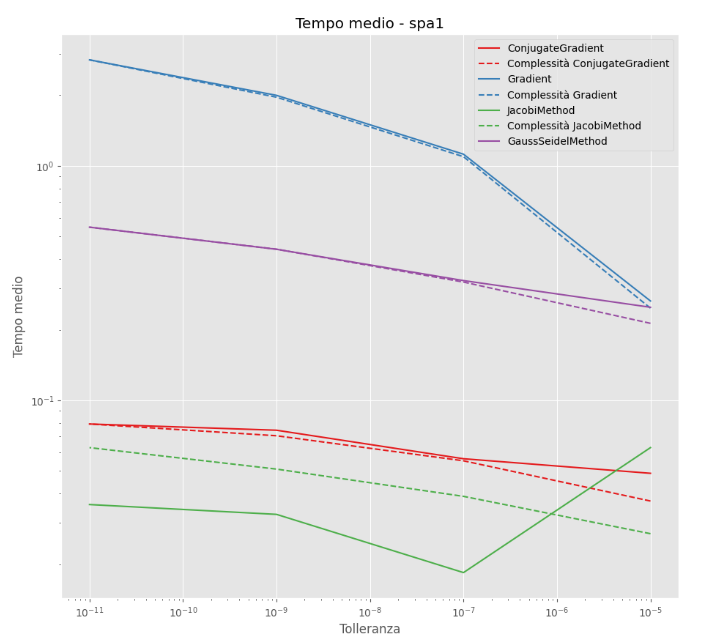
\includegraphics[width=\textwidth]{./../report/Progetto_1_bis/img/time_spa1.png}
        \caption{Matrice spa1}
        \label{fig:time_spa1}
    \end{subfigure}
    \hfill
    \begin{subfigure}{0.45\textwidth}
        \centering
        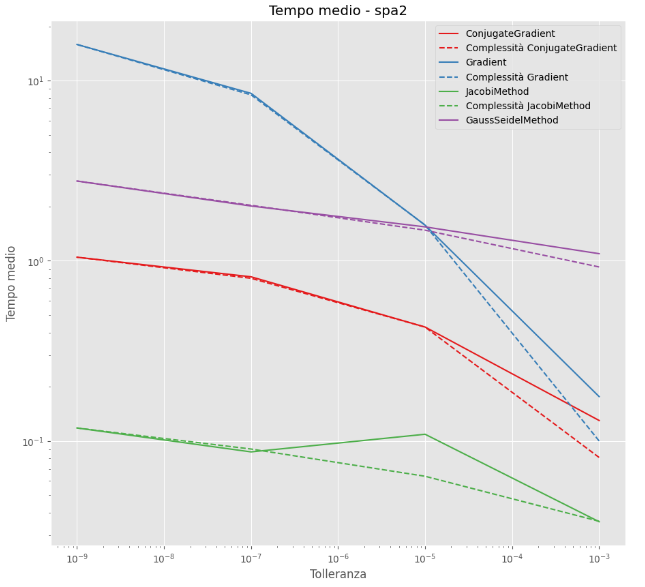
\includegraphics[width=\textwidth]{./../report/Progetto_1_bis/img/time_spa2.png}
        \caption{Matrice spa2}
        \label{fig:time_spa2}
    \end{subfigure}
    \hfill
    \begin{subfigure}{0.45\textwidth}
        \centering
        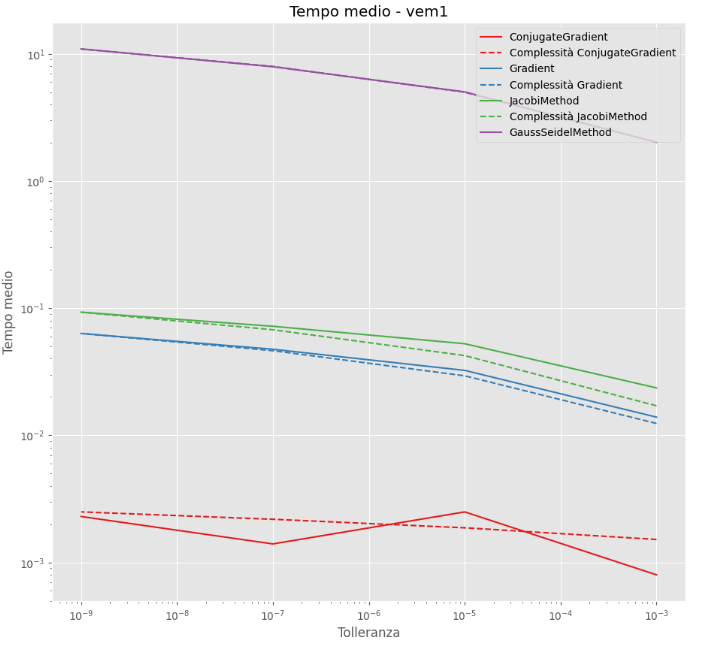
\includegraphics[width=\textwidth]{./../report/Progetto_1_bis/img/time_vem1.png}
        \caption{Matrice vem1}
        \label{fig:time_vem1}
    \end{subfigure}
    \hfill
    \begin{subfigure}{0.45\textwidth}
        \centering
        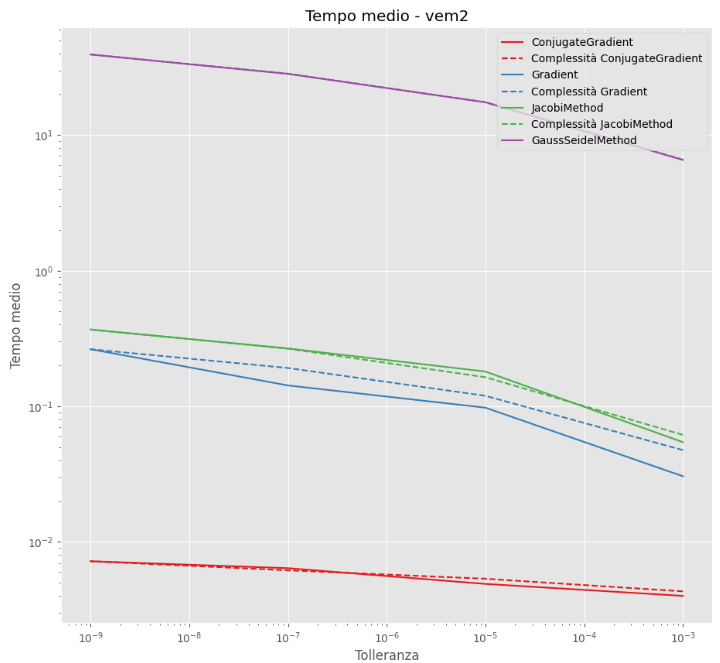
\includegraphics[width=\textwidth]{./../report/Progetto_1_bis/img/time_vem2.png}
        \caption{Matrice vem2}
        \label{fig:time_vem2}
    \end{subfigure}
    \caption{Tempi di esecuzione, in secondi, dei metodi iterativi. Le linee
        continue rappresentano i dati empirici, le linee tratteggiate rappresentano
        l'andamento teorico dei metodi.}
    \label{fig:time}
\end{figure}

In questi grafici, si può osservare che per tutte le implementazioni il tempo di
esecuzione aumenta man mano che la tolleranza si avvicina allo zero. Questo
comportamento è prevedibile, poiché il numero di iterazioni necessarie per
raggiungere la tolleranza aumenta, come evidenziato nella tabella \ref{tab:iterazioni}.
Inoltre, si nota che tutti i metodi tendono ad avere un andamento simile a quello
teorico.
\begin{table}[!ht]
    \centering
    \begin{subtable}[!ht]{1\textwidth}
        \centering
        \resizebox{\textwidth}{!}{\begin{tabular}{@{}ccccc|cccc@{}}
                \toprule
                \textbf{}                  & \multicolumn{4}{c|}{\textbf{spa1}} & \multicolumn{4}{c}{\textbf{spa2}}                                       \\ \midrule
                \textbf{tolleranza}        &
                \textbf{ConjugateGradient} &
                \textbf{GaussSeidelMethod} &
                \textbf{Gradient}          &
                \textbf{JacobiMethod}      &
                \textbf{ConjugateGradient} &
                \textbf{GaussSeidelMethod} &
                \textbf{Gradient}          &
                \textbf{JacobiMethod}                                                                                                                     \\ \midrule
                \textbf{0.0001}            & 49                                 & 10                                & 144   & 116 & 42  & 6  & 162  & 37  \\
                \textbf{1e-06}             & 134                                & 18                                & 3578  & 182 & 122 & 9  & 1950 & 58  \\
                \textbf{1e-08}             & 177                                & 25                                & 8234  & 248 & 196 & 13 & 5088 & 79  \\
                \textbf{1e-10}             & 200                                & 32                                & 12920 & 314 & 240 & 16 & 8286 & 100 \\ \bottomrule
            \end{tabular}}
        \caption{Spa 1 e Spa 2}
        \label{tab:spa}
    \end{subtable}
    \hfill
    \begin{subtable}[!ht]{1\textwidth}
        \centering
        \resizebox{\textwidth}{!}{\begin{tabular}{@{}ccccc|cccc@{}}
                \toprule
                \textbf{}                  & \multicolumn{4}{c|}{\textbf{vem1}} & \multicolumn{4}{c}{\textbf{vem2}}                                         \\ \midrule
                \textbf{tolleranza}        &
                \textbf{ConjugateGradient} &
                \textbf{GaussSeidelMethod} &
                \textbf{Gradient}          &
                \textbf{JacobiMethod}      &
                \textbf{ConjugateGradient} &
                \textbf{GaussSeidelMethod} &
                \textbf{Gradient}          &
                \textbf{JacobiMethod}                                                                                                                       \\ \midrule
                \textbf{0.0001}            & 38                                 & 660                               & 891  & 1315 & 47 & 966  & 1309 & 1928 \\
                \textbf{1e-06}             & 45                                 & 1219                              & 1613 & 2434 & 56 & 1841 & 2439 & 3677 \\
                \textbf{1e-08}             & 53                                 & 1779                              & 2337 & 3553 & 66 & 2715 & 3567 & 5426 \\
                \textbf{1e-10}             & 59                                 & 2339                              & 3059 & 4672 & 74 & 3590 & 4697 & 7175 \\ \bottomrule
            \end{tabular}}
        \caption{Vem 1 e Vem 2}
        \label{tab:vem}
    \end{subtable}
    \caption{Iterazioni}
    \label{tab:iterazioni}
\end{table}

Confrontando i vari metodi iterativi in base al tempo, il metodo di Gauß-Seidel
risulta essere il più lento per le matrici vem1 e vem2, nonostante il numero di
iterazioni sia inferiore rispetto ad altri metodi, come si può vedere nella tabella
\ref{tab:iterazioni}.
Questo è dovuto dal fatto che si richiede di risolvere un sistema lineare solo
per calcolare di quanto aggiornare la soluzione attuale.
Invece, per le matrici spa1 e spa2, il metodo che richiede più tempo è il metodo
del gradiente. Questo comportamento può essere attribuito al fatto che la convergenza
del metodo presenta un andamento a zig-zag. A supporto di questa ipotesi, si
osserva che il numero di condizionamento delle matrici spa1 e spa2 è molto elevato,
pari rispettivamente a 2048 e 1411. Pertanto, è plausibile che la combinazione
di un numero di condizionamento elevato e il punto di partenza scelto per il
metodo, ovvero il vettore nullo, conduca a un andamento a zig-zag nella convergenza.
Al contrario, il metodo di Jacobi risulta essere il più veloce per le matrici spa1
e spa2, mentre per le matrici vem1 e vem2 il più veloce è il gradiente coniugato.
Questo comportamento è dovuto principalmente dal numero di condizionamento che,
essendo alto per le matrici spa1 e spa2, rallenta l'esecuzione dei metodi basati
sul gradiente.

\begin{table}[!ht]
    \centering
    \begin{subtable}[!ht]{1\textwidth}
        \centering
        \resizebox{\textwidth}{!}{\begin{tabular}{@{}ccccc|cccc@{}}
                \toprule
                \textbf{}                  & \multicolumn{4}{c|}{\textbf{spa1}} & \multicolumn{4}{c}{\textbf{spa2}}                                                        \\ \midrule
                \textbf{tolleranza}        &
                \textbf{ConjugateGradient} &
                \textbf{GaussSeidelMethod} &
                \textbf{Gradient}          &
                \textbf{JacobiMethod}      &
                \textbf{ConjugateGradient} &
                \textbf{GaussSeidelMethod} &
                \textbf{Gradient}          &
                \textbf{JacobiMethod}                                                                                                                                      \\ \midrule
                \textbf{0.0001}            & 0.0565                             & 0.3456                            & 0.0774 & 0.1142 & 0.2315 & 1.2617 & 0.4155  & 0.0531 \\
                \textbf{1e-06}             & 0.0983                             & 0.5263                            & 1.3489 & 0.0411 & 0.6189 & 2.509  & 4.9883  & 0.0821 \\
                \textbf{1e-08}             & 0.0783                             & 0.7074                            & 3.1765 & 0.046  & 1.0987 & 2.5651 & 15.5589 & 0.1069 \\
                \textbf{1e-10}             & 0.0792                             & 0.552                             & 2.6059 & 0.0395 & 1.3551 & 3.5277 & 24.5388 & 0.1476 \\ \bottomrule
            \end{tabular}}
        \caption{Spa 1 e Spa 2}
        \label{tab:spa_time}
    \end{subtable}
    \hfill
    \begin{subtable}[!ht]{1\textwidth}
        \centering
        \resizebox{\textwidth}{!}{\begin{tabular}{@{}ccccc|cccc@{}}
                \toprule
                \textbf{}                  & \multicolumn{4}{c|}{\textbf{vem1}} & \multicolumn{4}{c}{\textbf{vem2}}                                                        \\ \midrule
                \textbf{tolleranza}        &
                \textbf{ConjugateGradient} &
                \textbf{GaussSeidelMethod} &
                \textbf{Gradient}          &
                \textbf{JacobiMethod}      &
                \textbf{ConjugateGradient} &
                \textbf{GaussSeidelMethod} &
                \textbf{Gradient}          &
                \textbf{JacobiMethod}                                                                                                                                      \\ \midrule
                \textbf{0.0001}            & 0.0022                             & 3.9035                            & 0.0324 & 0.0531 & 0.0039 & 13.5665 & 0.0651 & 0.1244 \\
                \textbf{1e-06}             & 0.0022                             & 7.1674                            & 0.0435 & 0.0723 & 0.007  & 25.9683 & 0.1639 & 0.1993 \\
                \textbf{1e-08}             & 0.0033                             & 10.5044                           & 0.0643 & 0.0989 & 0.005  & 36.1589 & 0.1671 & 0.4492 \\
                \textbf{1e-10}             & 0.0032                             & 13.9824                           & 0.0832 & 0.1281 & 0.0067 & 48.7597 & 0.2683 & 0.476  \\ \bottomrule
            \end{tabular}}
        \caption{Vem 1 e Vem 2}
        \label{tab:vem_time}
    \end{subtable}
    \caption{Tempo medio, espresso in secondi, di 10 esecuzioni}
    \label{tab:times}
\end{table}

Per quanto riguarda l'occupazione di memoria, i risultati ottenuti sono riportati
nelle figure \ref{fig:mem_spa1}, \ref{fig:mem_spa2}, \ref{fig:mem_vem1} e \ref{fig:mem_vem2}.

\begin{figure}[!ht]
    \centering
    \begin{subfigure}{0.45\textwidth}
        \centering
        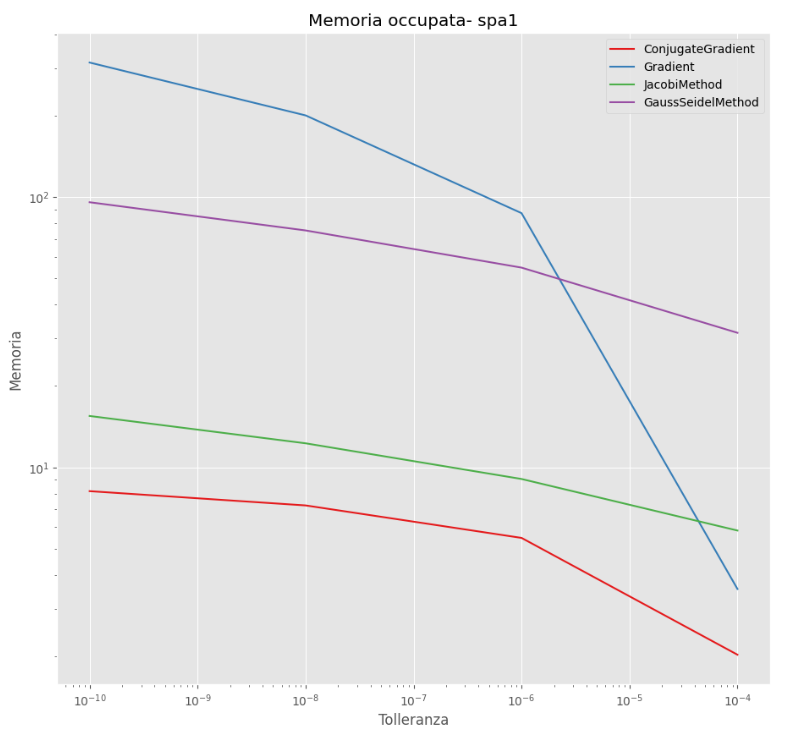
\includegraphics[width=\textwidth]{./../report/Progetto_1_bis/img/mem_spa1.png}
        \caption{Matrice spa1}
        \label{fig:mem_spa1}
    \end{subfigure}
    \begin{subfigure}{0.45\textwidth}
        \centering
        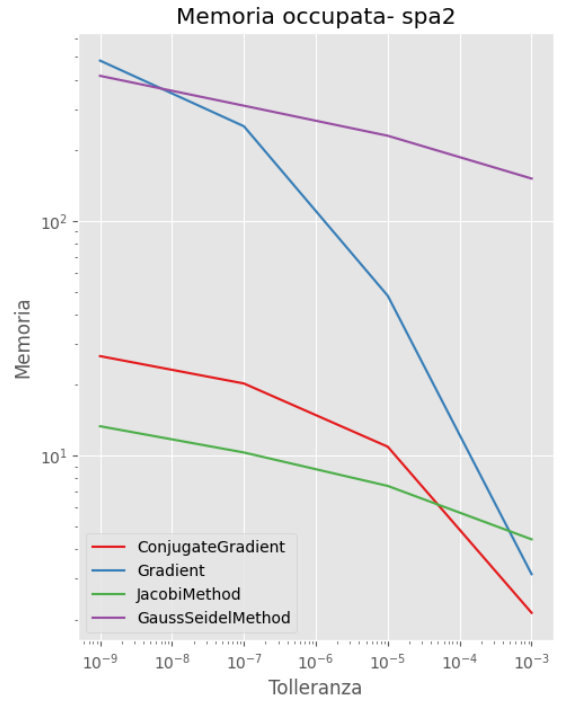
\includegraphics[width=\textwidth]{./../report/Progetto_1_bis/img/mem_spa2.png}
        \caption{Matrice spa2}
        \label{fig:mem_spa2}
    \end{subfigure}
    \begin{subfigure}{0.45\textwidth}
        \centering
        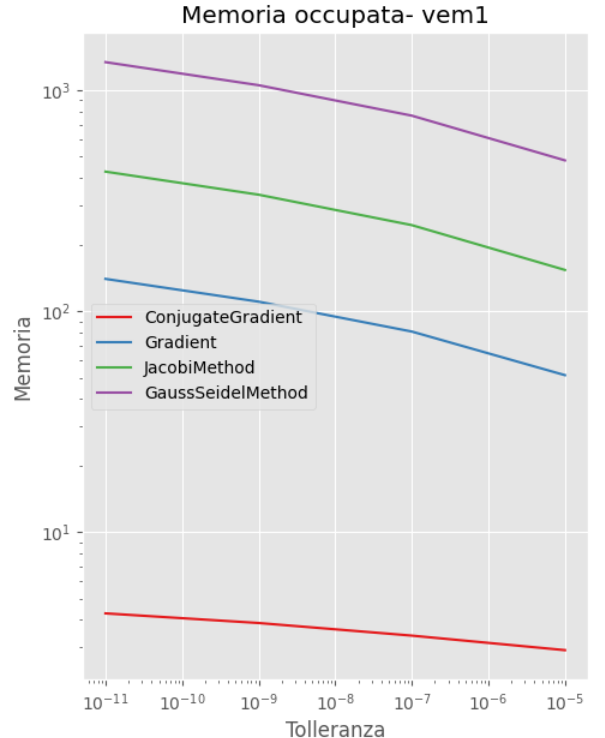
\includegraphics[width=\textwidth]{./../report/Progetto_1_bis/img/mem_vem1.png}
        \caption{Matrice vem1}
        \label{fig:mem_vem1}
    \end{subfigure}
    \begin{subfigure}{0.45\textwidth}
        \centering
        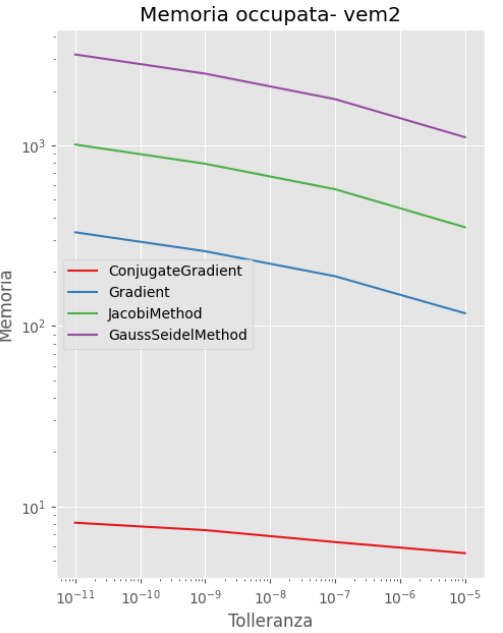
\includegraphics[width=\textwidth]{./../report/Progetto_1_bis/img/mem_vem2.png}
        \caption{Matrice vem2}
        \label{fig:mem_vem2}
    \end{subfigure}
    \caption{Memoria occupata, in MB, dei metodi iterativi.}
    \label{fig:memory}
\end{figure}

In questi grafici, possiamo notare lo spazio richiesto dai vari metodi cresce
all'aumentare del numero di iterazioni e, quindi, alla diminuzione della tolleranza
richiesta per la convergenza. In generale il metodo del gradiente coniugato richiede
meno memoria rispetto agli altri metodi nelle matrici spa1, vem1 e vem2; mentre per
la matrice spa2 il metodo che richiede meno memoria è Jacobi.

Infine, presentiamo i grafici che illustrano la variazione dell'errore medio in
funzione della tolleranza per ciascuna matrice, come mostrato nelle figure \ref{fig:error_spa1},
\ref{fig:error_spa2}, \ref{fig:error_vem1} e \ref{fig:error_vem2}.

\begin{figure}[!ht]
    \centering
    \begin{subfigure}{0.45\textwidth}
        \centering
        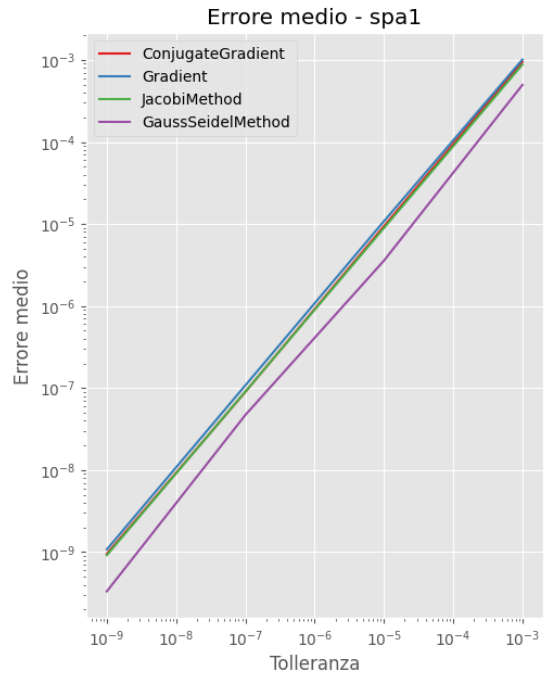
\includegraphics[width=\textwidth]{./../report/Progetto_1_bis/img/error_spa1.png}
        \caption{Matrice spa1}
        \label{fig:error_spa1}
    \end{subfigure}
    \begin{subfigure}{0.45\textwidth}
        \centering
        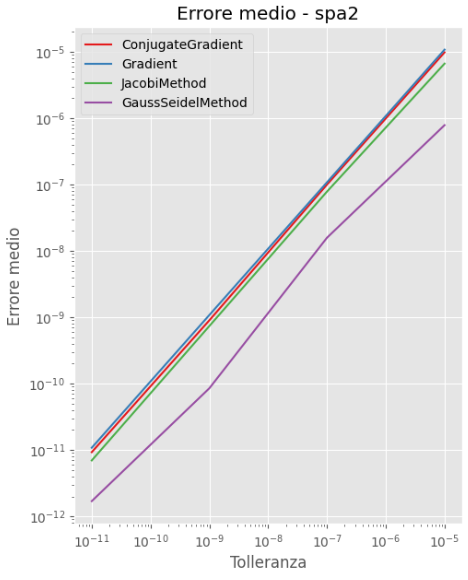
\includegraphics[width=\textwidth]{./../report/Progetto_1_bis/img/error_spa2.png}
        \caption{Matrice spa2}
        \label{fig:error_spa2}
    \end{subfigure}
    \begin{subfigure}{0.45\textwidth}
        \centering
        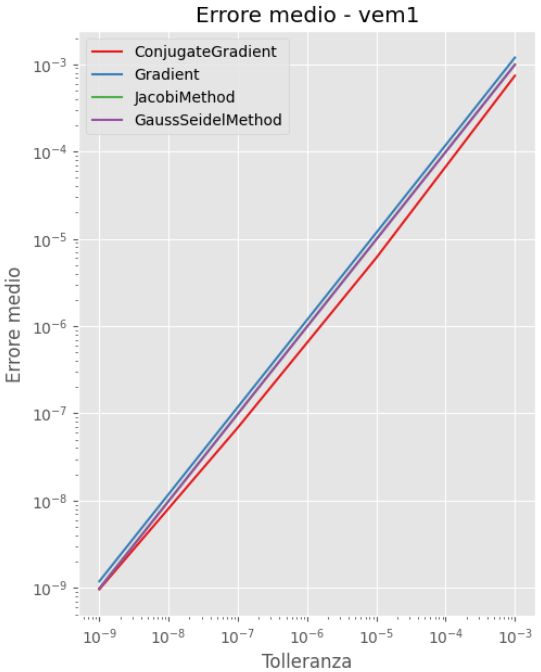
\includegraphics[width=\textwidth]{./../report/Progetto_1_bis/img/error_vem1.png}
        \caption{Matrice vem1}
        \label{fig:error_vem1}
    \end{subfigure}
    \begin{subfigure}{0.45\textwidth}
        \centering
        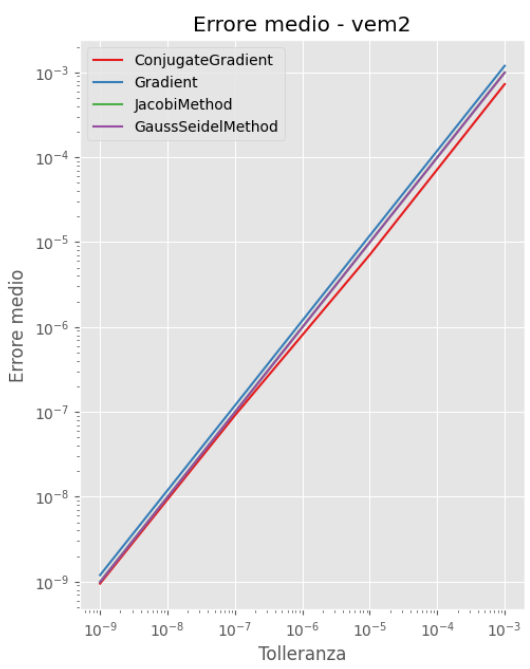
\includegraphics[width=\textwidth]{./../report/Progetto_1_bis/img/error_vem2.png}
        \caption{Matrice vem2}
        \label{fig:error_vem2}
    \end{subfigure}
    \caption{Errore dei metodi iterativi}
    \label{fig:error}
\end{figure}

In questi grafici possiamo osservare un andamento che decresce più la tolleranza
si avvicina a zero. Questo è legato al fatto che tutti i metodi implementati
convergono prima di raggiungere il numero di iterazioni massimo (20000). Inoltre,
non si riesce a notare una differenza significativa tra i metodi implementati in termini
di errore ottenuto.

\begin{table}[!ht]
    \centering
    \begin{subtable}[!ht]{1\textwidth}
        \centering
        \resizebox{\textwidth}{!}{
            \begin{tabular}{@{}ccccc|cccc@{}}
                \toprule
                \textbf{}                  & \multicolumn{4}{c|}{\textbf{spa1}} & \multicolumn{4}{c}{\textbf{spa2}}                                                                \\ \midrule
                \textbf{tolleranza}        &
                \textbf{ConjugateGradient} &
                \textbf{GaussSeidelMethod} &
                \textbf{Gradient}          &
                \textbf{JacobiMethod}      &
                \textbf{ConjugateGradient} &
                \textbf{GaussSeidelMethod} &
                \textbf{Gradient}          &
                \textbf{JacobiMethod}                                                                                                                                              \\ \midrule
                \textbf{0.0001}            & 2.024                              & 31.4718                           & 3.544    & 5.8335  & 5.1464  & 177.9521 & 11.7837  & 5.8432  \\
                \textbf{1e-06}             & 5.4784                             & 54.8552                           & 87.2787  & 9.0522  & 14.7656 & 257.0499 & 140.7772 & 8.8733  \\
                \textbf{1e-08}             & 7.226                              & 75.3157                           & 200.8106 & 12.2709 & 23.6634 & 362.5135 & 367.1651 & 11.9033 \\
                \textbf{1e-10}             & 8.1607                             & 95.7762                           & 315.074  & 15.4896 & 28.954  & 441.6113 & 597.8816 & 14.9334 \\ \bottomrule
            \end{tabular}}
        \caption{Spa 1 e Spa 2}
        \label{tab:spa_mem}
    \end{subtable}
    \hfill
    \begin{subtable}[!ht]{1\textwidth}
        \centering
        \resizebox{\textwidth}{!}{\begin{tabular}{@{}ccccc|cccc@{}}
                \toprule
                \textbf{}                  & \multicolumn{4}{c|}{\textbf{vem1}} & \multicolumn{4}{c}{\textbf{vem2}}                                                                  \\ \midrule
                \textbf{tolleranza}        &
                \textbf{ConjugateGradient} &
                \textbf{GaussSeidelMethod} &
                \textbf{Gradient}          &
                \textbf{JacobiMethod}      &
                \textbf{ConjugateGradient} &
                \textbf{GaussSeidelMethod} &
                \textbf{Gradient}          &
                \textbf{JacobiMethod}                                                                                                                                                \\ \midrule
                \textbf{0.0001}            & 2.6448                             & 338.0852                          & 36.4931  & 107.8292 & 4.9981 & 764.5668  & 82.2053  & 242.3596 \\
                \textbf{1e-06}             & 3.1219                             & 624.2216                          & 66.02    & 199.3544 & 5.9392 & 1456.7548 & 153.097  & 461.8102 \\
                \textbf{1e-08}             & 3.6672                             & 910.8699                          & 95.6287  & 290.8797 & 6.9848 & 2148.1518 & 223.8632 & 681.2607 \\
                \textbf{1e-10}             & 4.0761                             & 1197.5183                         & 125.1556 & 382.4049 & 7.8212 & 2840.3398 & 294.7549 & 900.7112 \\ \bottomrule
            \end{tabular}
        }
        \caption{Vem 1 e Vem 2}
        \label{tab:vem_mem}
    \end{subtable}
    \caption{Memoria utilizzata in MB}
    \label{tab:memory}
\end{table}

Infine risulta di notevole interesse segnalare che nessuna delle matrici sono a
dominanza diagonale, questo comporta che non viene rispettata la condizione sufficiente
di convergenza per i metodi Gauß Seidel e Jacobi, ma per tutte le tolleranze i metodi
hanno raggiunto la convergenza.

\begin{table}[!ht]
    \centering
    \begin{subtable}[!ht]{1\textwidth}
        \centering
        \resizebox{\textwidth}{!}{\begin{tabular}{@{}ccccc|cccc@{}}
                \toprule
                \textbf{}                  & \multicolumn{4}{c|}{\textbf{spa1}} & \multicolumn{4}{c}{\textbf{spa2}}                                                                                             \\ \midrule
                \textbf{tolleranza}        &
                \textbf{ConjugateGradient} &
                \textbf{GaussSeidelMethod} &
                \textbf{Gradient}          &
                \textbf{JacobiMethod}      &
                \textbf{ConjugateGradient} &
                \textbf{GaussSeidelMethod} &
                \textbf{Gradient}          &
                \textbf{JacobiMethod}                                                                                                                                                                           \\ \midrule
                \textbf{0.0001}            & 9.777927e-05                       & 4.210657e-05                      & 0.00010586318 & 8.840363e-05 & 9.913569e-05 & 1.172083e-05 & 0.00010630983 & 7.637818e-05 \\
                \textbf{1e-06}             & 9.742e-07                          & 3.0054e-07                        & 1.07831e-06   & 8.9734e-07   & 9.0899e-07   & 2.1278e-07   & 1.08195e-06   & 7.2076e-07   \\
                \textbf{1e-08}             & 9.03e-09                           & 3.95e-09                          & 1.08e-08      & 9.11e-09     & 9.6e-09      & 1.16e-09     & 1.08e-08      & 6.8e-09      \\
                \textbf{1e-10}             & 8e-11                              & 5e-11                             & 1.1e-10       & 9e-11        & 1e-10        & 2e-11        & 1.1e-10       & 6e-11        \\ \bottomrule
            \end{tabular}}
        \caption{Spa 1 e Spa 2}
        \label{tab:spa_error}
    \end{subtable}
    \hfill
    \begin{subtable}[!ht]{1\textwidth}
        \centering
        \resizebox{\textwidth}{!}{\begin{tabular}{@{}ccccc|cccc@{}}
                \toprule
                \textbf{}                  & \multicolumn{4}{c|}{\textbf{vem1}} & \multicolumn{4}{c}{\textbf{vem2}}                                                                                            \\ \midrule
                \textbf{tolleranza}        &
                \textbf{ConjugateGradient} &
                \textbf{GaussSeidelMethod} &
                \textbf{Gradient}          &
                \textbf{JacobiMethod}      &
                \textbf{ConjugateGradient} &
                \textbf{GaussSeidelMethod} &
                \textbf{Gradient}          &
                \textbf{JacobiMethod}                                                                                                                                                                          \\ \midrule
                \textbf{0.0001}            & 7.111298e-05                       & 9.851301e-05                      & 0.00011843361 & 9.952991e-05 & 9.188121e-05 & 9.926331e-05 & 0.0001192269 & 9.965874e-05 \\
                \textbf{1e-06}             & 8.9014e-07                         & 9.9068e-07                        & 1.18807e-06   & 9.9521e-07   & 8.54e-07     & 9.9075e-07   & 1.18578e-06  & 9.963e-07    \\
                \textbf{1e-08}             & 7.8e-09                            & 9.88e-09                          & 1.18e-08      & 9.95e-09     & 8.6e-09      & 9.94e-09     & 1.192e-08    & 9.96e-09     \\
                \textbf{1e-10}             & 7e-11                              & 1e-10                             & 1.2e-10       & 1e-10        & 6e-11        & 1e-10        & 1.2e-10      & 1e-10        \\ \bottomrule
            \end{tabular}}
        \caption{Vem 1 e Vem 2}
        \label{tab:vem_error}
    \end{subtable}
    \caption{Errore medio dei metodi iterativi}
    \label{tab:erors}
\end{table}
